\documentclass[12pt]{amsart}
\usepackage{graphicx}
\usepackage{amsthm}
\usepackage{tikz}
\usepackage{tikz-qtree}

\newcommand{\HRule}{\rule{\linewidth}{0.5mm}}
\newcommand{\n}{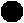
\includegraphics[width=0.35cm,height=0.35cm]{images/node}}

\newtheorem*{orderp}{Definition}
\newtheorem*{trees}{Definition}

\begin{document}
  \begin{titlepage}
  \centering
  
  \huge{\textbf{Runge-Kutta Methods with Rooted Trees}}
  \\[0.1cm]
  \HRule
  \vfill
  \begin{tikzpicture}
  \tikzset{level distance=80pt}
  \tikzset{sibling distance=60pt}
   \tikzset{grow'=up}
    \Tree [.\n{} ]
  \end{tikzpicture}
  \hfill
  \begin{tikzpicture}
  \tikzset{level distance=40pt}
  \tikzset{sibling distance=60pt}
   \tikzset{grow'=up}
    \Tree [.\n{} [ \n{} ]]
  \end{tikzpicture}
 \hfill
 \begin{tikzpicture}
  \tikzset{level distance=80pt}
  \tikzset{sibling distance=60pt}
   \tikzset{grow'=up}
    \Tree [.\n{} [ .\n{} ] [ .\n{} ] ]
  \end{tikzpicture}
  \hfill
  \begin{tikzpicture}
  \tikzset{level distance=80pt}
  \tikzset{sibling distance=60pt}
   \tikzset{grow'=up}
    \Tree [.\n{} [.\n{} \n{} ] ]
  \end{tikzpicture}
  \vfill
  \textsc{\large Wilfrid Laurier University}
  \\[0.1cm]
  \textsc{\large MA489 Interim Report}
  \HRule
  \\[0.5cm]
  
  \large \emph{Author:}
  \hfill
  \hfill
  \large \emph{Supervisor:}
  \\
  \large \textbf{Richard Douglas}
  \hfill
  \hfill
  \large \textbf{Dr. Shengda Hu}
  \\[2.0cm]
  \today{}
  \end{titlepage}

  \section[*]{\textbf{Introduction}}
  In the sciences and engineering, ordinary differential equations are often encountered when a 
  particular problem has been modeled mathematically. Solving the problem then requires solving 
  the ODEs but this cannot always be done analytically as it may not yet be known how to do so 
  or it may require a lot of effort. For this reason, numerical methods for solving ODEs are of 
  interest.

  A typical ODE has form 
  $$y'(x) = f(x,y) \mbox{ } \forall x \in [a,b],$$
  $$y(x_0) = y_0 \mbox{ for some } x_0 \in [a,b].$$
  Throughout this document, $f(x,y)$ is assumed to be infinitely differentiable.
  
  The problem then is to be able to approximate $y(x)$ for any given $x$ in the interval. This is 
  often done by splitting up the interval from $x_0$ to $x$ into subintervals 
  $[x_0, x_1], [x_1, x_2], \dots [x_{N-1},x_N]$ of equal width $h$ and then computing a 
  sequence of approximations from $y_n = y(x_n)$ to $y_{n+1} = y(x_{n+1})$ until 
  at last we have computed the approximation at the value $x_N$ which is the point at 
  which we wanted to approximate $y(x)$.

  There is a limit to how small we can make $h$ however, as if we make $h$ too small, the 
  computer runs into rounding error and our approximation is no good. This motivates the concept
  of order which tells us how fast the numerical method's approximation converges to the true 
  value of $y(x)$. 
  
  \begin{orderp} A method is said to be of \textbf{order p} if 
  $$\lim_{h \to 0} \frac{|y_N - y(x_N)|}{h^p} < \infty$$
  More compactly this is often denoted as $O(h^p)$.
  \end{orderp}

  Since $h$ is going to $0$, a higher order means that the approximation
  is converging faster to the true value.
  
  ~\\
  An example of a numerical method for solving ODEs is the \\
  \textbf{Euler method}:
  $$x_{n+1} = x_n + h$$
  $$y_{n+1} = y_n + hf(x_n,y_n)$$
  \\
  This is the most basic Runge-Kutta method but it does not converge quickly as it is only of order 
  1. \pagebreak

  \section{\textbf{Runge-Kutta methods}}
  The \textbf{Runge-Kutta methods} are a family of numerical algorithms for approximating the  
  solutions to ordinary differential equations. 
  The way Runge-Kutta methods are carried out is by splitting the interval into subintervals of 
  equal width $h$ as before and computing a sequence of approximations $y_n$. 

  In the step from $y_n$ to $y_{n+1}$ a number of intermediate approximations for $y$
  $$Y_1, Y_2, \dots Y_s$$ 
  at values of $x$ in $[x_n, x_{n+1}]$ are computed. These approximations are called 
  \textbf{stages} and $s$ denotes the number of stages. 
  
  Each stage's corresponding $x$ value in $[x_n, x_{n+1}]$ is denoted by
  $$X_1, X_2, \dots X_s$$
  where to be in the subinterval, $X_i = x_n + c_ih \mbox{ for some } c_i \in [0,1].$

  The \textbf{stage derivatives} are obtained by plugging $X_i$ and $Y_i$ into $f(x,y)$.
  $$f(X_1, Y_1), f(X_2, Y_2), \dots f(X_s, Y_s)$$
  The first $x$ value, stage, and stage derivative in a step are always
  $$X_1 = x_n \mbox{ (implying } c_1 = 0),  Y_1 = y_n, f(X_1, Y_1) = f(x_n, y_n)$$
  For explicit Runge-Kutta methods, each stage is computed using its preceding stage derivatives 
  as follows
  \begin{flalign*}
  Y_2 &= y_n + a_{21}hf(X_1,Y_1) = y_n + a_{21}hf(x_n,y_n) &\\ 
  &\\
  Y_3 &= y_n + a_{31}hf(X_1,Y_1) + a_{32}hf(X_2,Y_2) &\\
  &\\
  \vdots &\\
  Y_s &= y_n + \sum_{j=1}^{s-1}{a_{sj}hf(X_j,Y_j)} 
  \end{flalign*}
  where $a_{ij}$ is the coefficient corresponding to how state $Y_i$ 
  depends on stage derivative $f(X_j,Y_j)$.

  Once all stages have been computed, $y_{n+1}$ is approximated as being
  % $$y_{n+1} = y_n + hb_1f(X_1,Y_1) + hb_2f(X_2,Y_2) + \dots + hb_sf(X_s,Y_s)$$
  $$y_{n+1} = y_n + h\sum_{i = 1}^s{b_if(X_i,Y_i)}$$ 
  where the $b_i$ terms are known as the \textbf{weights}. 
  \pagebreak

  In summary, a Runge-Kutta method can be represented by a tableau of form
  \begin{table}[h]
  \centering
   \renewcommand{\arraystretch}{1.25}
     \begin{tabular}{r | c*{4}{c}}
                        $0$ \\
                    $c_2$ & $a_{21}$ \\
                    $c_3$ & $a_{31}$ & $a_{32}$ \\
                   $\vdots$ & $\vdots$      &  $\vdots$  & $\ddots$ \\
	        $c_s$ & $a_{s1}$  &  $a_{s2}$  & $\dots$ & $a_{s(s-1)}$\\
                     \hline
    \phantom{c4}     & $b_1$ & $b_2$ & $\dots$ & $b_s$ \\
    \end{tabular}
  \renewcommand{\arraystretch}{1.0}
  \end{table}
  
  Where
  \begin{itemize}
    \item $a_{ij}$ represents how stage $i$ depends on the $jth$ stage derivative,
    \item $b_i$ represents the weight of $hf(X_i,Y_i)$ in computing $y_{n+1}$,
    \item $c_i$ represents the location of $X_i$ in the interval $[x_n,x_{n+1}]$
  \end{itemize}
  ~\\

  \section[*]{\textbf{Deriving Runge-Kutta methods}}
  In order for a Runge-Kutta method to be of order $p$, at least $s = p$ stages are necessary.
  there is also a system of equations which the parameters must satisfy.
  The usual way to derive these equations is by first choosing the number of stages to use, 
  writing the method in its most general form, and then solving for the parameters by comparing 
  the Taylor expansion of the method with that of the order $p$ \textbf{Taylor method} given by
  $$y_{n+1} = y_n + f(x_n,y_n)h + \frac{f'(x_n,y_n)h^2}{2!} + \dots + \frac{f^{(p-1)}
      (x_n,y_n)h^p}{p!}.$$

  One major reason why Runge-Kutta methods are favoured over Taylor methods is that 
  implementing the Taylor method requires taking derivatives of $f(x,y)$ with respect to $x$. 
  These derivatives grow very complicated as $p$ increases
  $$f'(x,y) = f_x(x,y) + f_y(x,y)f(x,y)$$
  $$f''(x,y) = f_{xx} + 2f_{xy}f + f_yf_x + f_{yy}f^2 + f_y^2f$$
  $$f'''(x,y) = f_{xxx} + 3f_{xxy}f + 3f_{xyy}f^2 + f_{yyy}f^3 + $$
  $$f_y(f_{xx} + 2f_{xy}f + f_{yy}f^2) +  3(f_x + f_yf)(f_{xy} + f_{yy}f) + f_y^2(f_x +  
      f_yf)$$
  $$\dots$$
  and so it is not very practical to code high order Taylor methods into a computer.
  
  As an example, the Runge-Kutta methods of order $2$ with two stages will be derived.
  These methods have X values
  $$X_1 = x_n, X_2 = x_n + c_2h,$$
  stages
  $$Y_1 = y_n, Y_2 = y_n + a_{21}hf(x_n,y_n),$$
  and stage derivatives
  $$f(X_1,Y_1) = f(x_n,y_n),$$ 
  $$f(X_2,Y_2) = f(x_n + c_2h, y_n + a_{21}hf(x_n,y_n)).$$
  The order $2$ methods with two stages can thus be represented compactly
  $$y_{n+1} = y_n + hb_1f(x_n,y_n) + hb_2f(x_n + c_2h,y_n + a_{21}hf(x_n,y_n)).$$
  The order $2$ Taylor method is
  $$y_{n+1} = y_n + f(x_n,y_n)h + \frac{f'(x_n,y_n)h^2}{2!}.$$
  The Taylor expansions of the methods are thus
  \begin{flalign*}
  y(x_{n+1}) &= y_n + b_1hf + b_2hf + b_2c_2h^2f_x + b_2a_{21}h^2f_yf + O(h^3), &\\
  y(x_{n+1}) &= y_n + hf + \frac{h^2f_x}{2} + \frac{h^2f_yf}{2} + O(h^3).
  \end{flalign*}
  Equating coefficients gives us the system of equations
  $$b_1 + b_2 = 1$$
  $$b_2c_2 = \frac{1}{2}$$
  $$b_2a_{21} = \frac{1}{2}$$
  Letting $b_2$ be a free parameter, all order $2$ Runge-Kutta methods with 
  two stages are of form
  \begin{table}[h]
  \centering
  \renewcommand{\arraystretch}{1.0}
     \begin{tabular}{r | c*{2}{c}}
                        $0$ \\
                    $\frac{1}{2b_2}$ & $\frac{1}{2b_2}$ \\
                     \hline
    \phantom{c4}     & $1 - b_2$ & $b_2$
    \end{tabular}
  \renewcommand{\arraystretch}{1.0}
  \end{table}
  
  Special cases include $b_2 = 1$ which gives us the \textbf{Midpoint method} 
  $$y_{n+1} = y_n + hf(x_n + \frac{h}{2}, y_n + \frac{h}{2}f(x_n,y_n))$$
  and $b_2 = \frac{1}{2}$ which corresponds to \textbf{Heun's method}.
  $$y_{n+1} = y_n + \frac{h}{2}f(x_n,y_n) + \frac{h}{2}f(x_n + h, y_n + hf(x_n,y_n))$$
  \pagebreak

  The problem with deriving Runge-Kutta methods this way is that it becomes increasingly more
  complicated as the required order increases. This is because we would need more stages which 
  when written in their general form will rely on more previously computed stage derivatives. 
  Higher derivatives of $f(x,y)$ for the Taylor method and Runge-Kutta method's Taylor 
  expansion would also be required.

  However it turns out that there is a way to derive the system of equations without having to
  deal with complicated Taylor expansions. With the equations known, values for the parameters
  can then be found and Runge-Kutta methods of the required order can then be implemented.

   \section[*]{\textbf{Rooted Trees}}
   \begin{trees}
   Rooted trees are directed graphs with a finite number of vertices such that every vertex has
  exactly one edge directed at it. There is one vertex, called the \textbf{root}, which breaks this
  rule and has no edges directed at it. Rooted trees are also connected and are typically drawn
  with their root vertex at the bottom of the illustration.
   \end{trees}
  
  \begin{tikzpicture}
   \tikzset{grow'=up}
   \tikzset{level distance=40pt}
   \tikzset{sibling distance=20pt}
    \Tree [.\n{} [.\n{} ]  [.\n{} \n{} ] ]
  \end{tikzpicture}
  \hfill
  \begin{tikzpicture}
   \tikzset{grow'=up}
  % \tikzset{level distance=80pt}
   %\tikzset{sibling distance=60pt}
   \tikzset{level distance=40pt}
   \tikzset{sibling distance=20pt}
    \Tree [.\n{} [.\n{} \n{} ]  [.\n{} ] ]
  \end{tikzpicture}
  
  Even though rooted trees are directed graphs, they are drawn without arrows and the direction
  of each edge goes from bottom to top with the root being the vertex at the very bottom of the 
  graph. Vertices that have no edges directed towards any other vertices (i.e. vertices at the top 
  of the tree), are known as \textbf{leaves}. 

  Trees that are order-isomorphic (that is, between which a bijection that preserves edges 
  exists ), such as the two trees depicted above, are treated as being equivalent. 
  %\pagebreak

  For a given rooted tree $t$, the following quantities are of interest:
  \begin{itemize}
    \item $r(t)$, (the \textbf{order} of $t$), the number of vertices in the tree,
    \item $\sigma(t)$, (the \textbf{symmetry} of $t$), the number of order-isomorphisms 
             from the tree to itself,
    \item $\gamma(t)$, this is defined to be the value obtained by taking the order of each 
             subtree that would be formed if each vertex of the tree were the root (not counting
             the vertices not at or above the vertex) and then multiplying all of these orders together.
   \item $\alpha(t)$, the number of ways to label the vertices of the tree using elements from the
            set $\left\{ 1, 2, \dots, r(t) \right\}$ such that
            \begin{itemize}
	 \item each vertex is only labeled once,
	 \item order-isomorphic labelings are only counted once,
	 \item if $(i, j)$ is a labeled edge directed from $i$ to $j$, 
                    then $i < j$.
            \end{itemize}
   \item $\beta(t)$, this is the same as $\alpha(t)$ except labelings need not 
	  satisfy the third condition.
  \end{itemize}

  \section[*]{\textbf{Deriving methods with Rooted Trees}}
  The Runge-Kutta methods of order 4 with four stages have equations 
  that correspond to the following trees:
  
  $$b_1 + b_2 + b_3 + b_4 = 1$$
  \hfill
  \begin{tikzpicture}
     \tikzset{grow'=up}
     \tikzset{level distance=40pt}
     \tikzset{sibling distance=30pt}
     \Tree [ .\n{} ]
  \end{tikzpicture}

  $$b_1c_1 + b_2c_2 + b_3c_3 + b_4c_4 = \frac{1}{2}$$
  \begin{tikzpicture}
    \tikzset{grow'=up}
    \tikzset{level distance=40pt}
     \tikzset{sibling distance=20pt}
    \Tree [.\n{} [.\n{} ] ]
  \end{tikzpicture}  
  \hfill
  
  $$b_1c_1^2 + b_2c_2^2 + b_3c_3^2 + b_4c_4^2 = \frac{1}{3}$$
  \hfill
  \begin{tikzpicture}
    \tikzset{grow'=up}
    \tikzset{level distance=40pt}
     \tikzset{sibling distance=20pt}
    \Tree [.\n{} [.\n{} ] [.\n{} ] ]
  \end{tikzpicture}

  $$b_1c_1^3 + b_2c_2^3 + b_3c_3^3 + b_4c_4^3 = \frac{1}{4}$$  
   \begin{tikzpicture}
    \tikzset{grow'=up}
    \tikzset{level distance=40pt}
     \tikzset{sibling distance=20pt}
    \Tree [.\n{} [.\n{} ] [.\n{} ] [.\n{} ] ] 
  \end{tikzpicture}
  \hfill

  \pagebreak
  $$\sum_{i, j=1}^s{b_ia_{ij}c_j} = \frac{1}{6}$$
  \hfill
  \begin{tikzpicture}
   \tikzset{grow'=up}
   \tikzset{level distance=40pt}
   \tikzset{sibling distance=20pt}
    \Tree [.\n{} [.\n{} \n{} ] ]
  \end{tikzpicture}

  $$\sum_{i, j=1}^s{b_ic_ia_{ij}c_j} = \frac{1}{8}$$
  \begin{tikzpicture}
   \tikzset{grow'=up}
   \tikzset{level distance=40pt}
   \tikzset{sibling distance=20pt}
    \Tree [.\n{} [.\n{} ]  [.\n{} \n{} ]]
  \end{tikzpicture}
  \hfill
  
  $$\sum_{i, j, k=1}^s{b_ia_{ij}a_{jk}c_k} = \frac{1}{24}$$
  \hfill
  \begin{tikzpicture}
   \tikzset{grow'=up}
   \tikzset{level distance=40pt}
   \tikzset{sibling distance=20pt}
    \Tree [.\n{} [.\n{} [.\n{} [ .\n{} ] ] ] ]
  \end{tikzpicture}

  \pagebreak
  $$\sum_{i, j=1}^s{b_ia_{ij}c_j^2} = \frac{1}{12}$$
  \begin{tikzpicture}
   \tikzset{grow'=up}
   \tikzset{level distance=40pt}
   \tikzset{sibling distance=20pt}
    \Tree [.\n{} [.\n{} \n{} \n{} ] ]
  \end{tikzpicture}
  \hfill

  From these diagrams it can be seen that by taking the rooted trees of orders
  ranging from 1 to 4, one can derive the system of equations that the parameters must satisfy. 
  For each tree $t$, one 
  starts at the bottom and writes $b_i$ for the root. 
  When a leaf is reached, $c_k$ is written down where $k$
  is the trailing letter of the leaf's preceding vertex. For intermediate vertices $a_{mn}$ is written
  where $m$ is the trailing letter of the preceding vertex and $n$ is a new letter. The terms 
  written down are then multiplied together and summed over all possible values that the letters 
  can take on.

  The preceding summation gives the lefthandside of the tree's equation. The righthandside is
  computed as being $1$ divided by $\gamma(t)$.
  
  \section[*]{\textbf{Conclusion}}
  The goal of the project is to understand (with proof) how to use rooted trees to
  derive the system of equations for Runge-Kutta methods of a given order.

  I may also look at the group formed by these trees (known as the \textbf{Butcher group})
  in which Runge-Kutta methods are obtained by doing compositions with methods of lower 
  orders.

  \section[*]{\textbf{References}}
  \begin{itemize} \item Butcher, John C., \textit{Numerical Methods for Ordinary Differential   
  Equations} (2008), second edition,
  \item Nagle et al., \textit{Fundamentals of Differential Equations and Boundary Value Problems}
           (2012), sections 3.6 and 3.7, sixth edition,
  \item Matthews, John H. and Fink, Kurtis D., \textit{Numerical Methods using Matlab} (2004),
           sections 9.4 and 9.5, fourth edition. 
  \end{itemize}
  
\end{document}